\documentclass[aspectratio=169]{beamer}

\usepackage[T1]{fontenc}
\usepackage[utf8]{inputenc}
\usepackage[american]{babel}
\usepackage{amsmath,amsthm}
\usepackage{multirow}
\usepackage{tikz}
\usetikzlibrary{matrix,decorations,decorations.text,calc,arrows,snakes,shapes,positioning}
\usepackage{multimedia}

\usepackage[nosfdefault]{comicneue}
\usepackage{sourcesanspro}
\usepackage[amssymb,amsfonts]{concmath}
\usefonttheme[onlymath]{serif}
\usepackage{ulem}

\mode<presentation>{%
  \usetheme{ibm}
}

\newcommand{\F}{\mathbb{F}}
\newcommand{\Z}{\mathbb{Z}}
\newcommand{\Q}{\mathbb{Q}}
\DeclareMathOperator{\End}{End}
\DeclareMathOperator{\Cl}{Cl}
\DeclareMathOperator{\poly}{poly}
\DeclareMathOperator{\polylog}{polylog}


\title[VDFs from Isogenies and Pairings]{Verifiable Delay Functions and More from Isogenies and Pairings}
\author[Luca De Feo]{
  Luca De Feo\\[1em]
  based on joint work with J.~Burdges, S.~Masson, C.~Petit, A.~Sanso}
\date[\url{https://defeo.lu/docet}~~~~~~ECC 2019]{December 4, 2019, ECC, Bochum\\
  \medskip
  Slides online at \url{https://defeo.lu/docet}}
\institute{IBM Research Zürich}

\begin{document}

\frame[plain]{\titlepage}

% {
%   \setbeamercolor{background canvas}{bg=black}
%   \begin{frame}[plain]
%     \begin{tikzpicture}[remember picture,overlay]
%       \node(pic)[at=(current page.center)] {
%         \includegraphics[width=\paperwidth]{pool.jpg}
%       };
%     \end{tikzpicture}
%   \end{frame}
  
%   %% 
  
%   \begin{frame}[plain]
%     \begin{tikzpicture}[remember picture,overlay]
%     \node(pic)[at=(current page.center)] {
%       \includegraphics[width=\paperwidth]{hodl.jpg}
%       };
%     \end{tikzpicture}
%   \end{frame}
% }

%% 

\begin{frame}{Distributed lottery}
  Participants \textbf{A, B, \dots, Z} want to agree on a random
  winning ticket.

  \begin{block}{Flawed protocol}
    \begin{itemize}
    \item Each participant \emph{$x$} broadcasts a random string
      \emph{$s_x$};
    \item Winning ticket is \emph{$H(s_A, \dots, s_Z)$}.
    \end{itemize}

    \pause
    
    Cheating participant \textbf{Z} waits to see all other strings,
    then brute-forces \emph{$s_Z$} to win lottery.
  \end{block}
  
  \pause

  \begin{block}{Fixes}
    \begin{itemize}
    \item Make the hash function \textbf{sloooooooooooooooooooooooooooow};
      \begin{itemize}
      \item e.g., participants have 10 minutes to submit $s_x$,
      \item outcome will be known after 20 minutes.
      \end{itemize}
    \item<4-> Make it possible to verify \emph{$w = H(s_A, \dots, s_Z)$} \textbf{fast}.
    \end{itemize}
  \end{block}
\end{frame}

%%

\begin{frame}{Verifiable Delay Functions (Boneh, Bonneau, Bünz, Fisch 2018)}
  \begin{block}{Wanted}
    Function (family) \emph{$f:X\to Y$} s.t.:

    \begin{itemize}
    \item Evaluating $f(x)$ takes \emph{long time}:
      \begin{itemize}
      \item \emph{uniformly} long time,
      \item on almost all random inputs $x$,
      \item even after having seen many values of $f(x')$,
      \item even given \emph{massive number of processors};
      \end{itemize}
    \item Verifying $y=f(x)$ is \emph{efficient}:
      \begin{itemize}
      \item ideally, exponential separation between evaluation and
        verification.
      \end{itemize}
    \end{itemize}
  \end{block}

  \centering
  \pause\vfill
  \textbf{Exercise}
  \pause\vfill
  Think of a function you like with these properties
  \pause\vfill
  Got it?
  \pause\vfill
  \textbf{You're probably wrong!}
\end{frame}

%%

\begin{frame}{Sequentiality}
  Ideal functionality:

  \[y = f(x) = \underbrace{H(H(\cdots(H(x))))}_{T \text{ times}}\]

  \begin{itemize}
  \item \emph{Sequential} assuming hash output ``unpredictability'',
  \item but how do you verify? \textcolor{gray}{(you're not allowed to say ``SNARKs'')}
  \end{itemize}
\end{frame}

%%

\begin{frame}{VDFs from groups of unknown order
    {\small (inspired by Rivest--Shamir--Wagner \emph{time-lock puzzle})}}
  \begin{columns}
    \begin{column}{0.6\textwidth}
      \begin{block}{Setup}
        A group of \emph{unknown order}, e.g.:
        \begin{itemize}
        \item \emph{$\Z/N\Z$} with $N=pq$ an RSA modulus, $p,q$ \emph{unknown}\\
          (e.g., generated by some trusted authority),
        \item \emph{Class group} of imaginary quadratic order.
        \end{itemize}
      \end{block}

      \begin{block}{Evaluation}
        With \emph{delay parameter} $T$:
        \begin{align*}
          f:G &\longrightarrow G\\
          x &\longmapsto x^{2^T}
        \end{align*}
        Conjecturally, fastest algorithm is repeated squaring.
      \end{block}
    \end{column}
    \begin{column}{0.37\textwidth}
      \only<-5>{
        \centering
        \begin{tikzpicture}[x=2cm,y=2cm]
          \def\crater{29}
          \draw[fill] (360/\crater:1) circle (1pt) +(360/\crater:1em) node {$x$};
          \uncover<2->{
            \draw[fill] (360/\crater : 1) -- (360/\crater*2 : 1)
            circle (1pt) +(360/\crater*2:1em) node {$x^2$};
          }
          \uncover<3->{
            \draw[fill] (360/\crater*2 : 1) -- (360/\crater*3 : 1)
            circle (1pt) +(360/\crater*3:1em) node {$x^4$};
          }
          \uncover<4->{
            \draw[dotted] (360/\crater*3 : 1) arc (360/\crater*3:360/\crater*23:1);
            \draw[fill] (360/\crater*23 : 1) circle (1pt) +(360/\crater*23:1em) node {$x^{2^T}$};
          }
          \uncover<5->{
            \draw[red] (360/\crater : 1) -- node[auto] {$2^T\bmod N$} (360/\crater*23 : 1);
          }
        \end{tikzpicture}
      }
      \only<6->{
        \begin{block}{Verification}
          Interactive proofs that \emph{$y=f(x)$},\\
          \textcolor{gray}{(non interactivity via Fiat-Shamir)}:

          \smallskip
          \begin{uncoverenv}<7->
            \textbf{Pietrzak '19:}
            \begin{itemize}
            \item Proof size \emph{$O(\log(T))$},
            \item Hard to find (non-trivial) \emph{$w\in G$ of known order}\\
              $\Rightarrow$ Proof is sound.
            \end{itemize}
          \end{uncoverenv}

          \smallskip
          \begin{uncoverenv}<8->
            \textbf{Wesolowski '19:}
            \begin{itemize}
            \item Proof size \emph{$O(1)$},
            \item More emph{ad hoc} security assumption.
            \end{itemize}
          \end{uncoverenv}
        \end{block}
      }
    \end{column}
  \end{columns}
\end{frame}

%%

\begin{frame}{Where have I seen this before?}
  \begin{columns}
    \begin{column}{0.6\textwidth}
      \begin{uncoverenv}<2->
        \begin{block}{Isogeny cycles}
          \begin{itemize}
          \item Vertices are \emph{elliptic curves}:
            \begin{itemize}
            \item Ordinary,
              \hfill\uncover<4->{\emph{Couveignes--Rostovtsev--Stolbunov}}
            \item Supersingular $/\F_p$.
              \hfill\uncover<4->{\emph{CSIDH}}
            \end{itemize}
          \item Edges are \emph{horizontal isogenies}.
          \item<3-> The \emph{class group} of $\End(E)$ acts upon the
            cycle:

            \smallskip
            \begin{tabular}{r c l}
              isogeny & ~$\leftrightarrow$~ & ideal\\
              endomorphism  & ~$\leftrightarrow$~ & principal ideal\\
              degree & ~$\leftrightarrow$~ & norm\\
              dual & ~$\leftrightarrow$~ & complex conjugate\\
              cycle size & ~$\leftrightarrow$~ & order of the ideal
            \end{tabular}
          \end{itemize}
        \end{block}
      \end{uncoverenv}
    \end{column}
    \begin{column}{0.4\textwidth}
      \centering
      \begin{tikzpicture}[x=2cm,y=2cm]
        \def\crater{17}
        \foreach \i in {0,...,\crater - 1} {
          \draw[fill] (360/\crater*\i:1) circle (1pt)
          +(360/\crater*\i:1em) node {\alt<2->{$E_{\i}$}{$x^{2^{\i}}$}};
          \draw (360/\crater*\i : 1) edge[bend right] (360/\crater*\i+360/\crater : 1);
        }
      \end{tikzpicture}
    \end{column}      
  \end{columns}
\end{frame}

%%

\begin{frame}{Slooooooooooooooooooooooooooooooooooooooooooow isogenies}
  \begin{columns}
    \begin{column}{0.6\textwidth}
      \begin{block}{Setup}
        With \emph{delay parameter} $T$:
        \begin{itemize}
        \item A laaaaaaaaaaaaaaaaaaaaaaaarge isogeny cycle,
        \item<2-> A \emph{starting curve} $E_0$,
        \item<2-> An isogeny \emph{$\phi:E_0\to E_T$} of degree \emph{$2^T$}.
        \end{itemize}
      \end{block}

      \begin{uncoverenv}<3->
        \begin{block}{Evaluation}
          $\phi$ \textbf{is} the VDF:
          \begin{align*}
            \phi:E_0(\F_p) &\longrightarrow E_T(\F_p)\\
            P &\longmapsto \phi(P)
          \end{align*}
          Conjecturally, no faster way than \emph{composing degree $2$
            isogenies}.
        \end{block}
      \end{uncoverenv}
    \end{column}
    \begin{column}{0.37\textwidth}
      \centering
      \begin{tikzpicture}[x=2cm,y=2cm]
        \def\crater{29}
        \draw[fill] (360/\crater:1) circle (1pt) +(360/\crater:1em) node {$E_0$};
        \draw[fill] (360/\crater : 1) -- (360/\crater*2 : 1)
        circle (1pt) +(360/\crater*2:1em) node {$E_1$};
        \draw[fill] (360/\crater*2 : 1) -- (360/\crater*3 : 1)
        circle (1pt) +(360/\crater*3:1em) node {$E_2$};
        \draw[dotted] (360/\crater*3 : 1) arc (360/\crater*3:360/\crater*23:1);
        \draw[fill] (360/\crater*23 : 1) circle (1pt) +(360/\crater*23:1em) node {$E_T$};
        \uncover<4->{
          \draw (0,0) node[anchor=center] {\Large\alert{How to verify?}};
        }
      \end{tikzpicture}
    \end{column}
  \end{columns}  
\end{frame}

%%

\begin{frame}{Isogeny <3 Pairing}
  \begin{block}{Theorem}
    Let \emph{$\phi:E\to E'$} be an isogeny and \emph{$\hat{\phi}:E' \to E$} its dual.
    Let \emph{$e_N$} be the Weil pairing of $E$ and \emph{$e_N'$} that
    of $E'$. %
    Then
    \[e_N(P,\hat{\phi}(Q)) = e_N'(\phi(P),Q),\]
    for any \emph{$P\in E[N]$} and \emph{$Q\in E'[N]$}.
  \end{block}
  
  \begin{block}{Corollary}
    \[e_N'(\phi(P),\phi(Q)) = e_N(P,Q)^{\deg\phi}.\]
  \end{block}
\end{frame}

%%

\begin{frame}{Refresher: Boneh--Lynn--Shacham (BLS) signatures}
  \begin{block}{}
    \begin{description}
    \item[Setup:]
      \begin{itemize}
      \item Elliptic curve $E/\F_p$, s.t \emph{$N|\#E(\F_p)$} for a large prime $N$,
      \item (Weil) pairing \emph{$e_N:E[N]\times E[N]\to\F_{p^k}$} for
        some small embedding degree $k$,
      \item A decomposition \emph{$E[N]=X_1 \times X_2$}, with
        \emph{$X_1=\langle P\rangle$}.
      \item A hash function \emph{$H:\{0,1\}^*\to X_2$}.
      \end{itemize}
    \item[Private key:] $s\in\Z/N\Z$.
    \item[Public key:] $sP$.
    \item[Sign:] $m \mapsto sH(m)$.
    \item[Verifiy:] $e_N(P,sH(m)) = e_N(sP,H(m))$.
    \end{description}
  \end{block}

  \centering
  \begin{tikzpicture}[ampersand replacement=\&]
    \matrix(m)[matrix of math nodes,row sep=3em,column sep=4em]{
      X_1 \times X_2 \& X_1 \times X_2\\
      X_1 \times X_2 \& \F_{p^k}\\
    };
    \draw[->]
    (m-1-1) edge node[above]{\small$[s]\times 1$} (m-1-2)
    (m-1-1) edge node[left]{\small$1\times [s]$} (m-2-1)
    (m-1-2) edge node[right]{\small$e_N$} (m-2-2)
    (m-2-1) edge node[below]{\small$e_N$} (m-2-2);
  \end{tikzpicture}
\end{frame}

%%

\begin{frame}{US patent 8,250,367 (Broker, Charles and Lauter 2012)}
  \begin{block}{Signatures from isogenies + pairings}
    \begin{itemize}
    \item Replace the secret \emph{$[s]:E\to E$} with an isogeny \emph{$\phi:E\to E'$};
    \item Define decompositions
      \begin{align*}
        E[N] = X_1 \times X_2, \qquad E'[N] = Y_1 \times Y_2,
      \end{align*}
      s.t. \emph{$\phi(X_1) = Y_1$} and \emph{$\phi(X_2) = Y_2$};
    \item Define a hash function \emph{$H:\{0,1\}^*\to Y_2$}.
    \end{itemize}
  \end{block}
  
  \centering
  \begin{tikzpicture}[ampersand replacement=\&]
    \matrix(m)[matrix of math nodes,row sep=3em,column sep=4em]{
      X_1 \times Y_2 \& Y_1 \times Y_2\\
      X_1 \times X_2 \& \F_{p^k}\\
    };
    \draw[->]
    (m-1-1) edge node[above]{\small$\phi\times 1$} (m-1-2)
    (m-1-1) edge node[left]{\small$1\times\hat{\phi}$} (m-2-1)
    (m-1-2) edge node[right]{\small$e_N'$} (m-2-2)
    (m-2-1) edge node[below]{\small$e_N$} (m-2-2);
  \end{tikzpicture}
\end{frame}

%%

\begin{frame}{Isogeny VDF {\small (principle)}}
  \begin{block}{Setup}
    \begin{itemize}
    \item Pairing friendly curve \emph{$E$},
    \item Isogeny \emph{$\phi:E\to E'$} of degree \emph{$\ell^T$},
    \item Point \emph{$P\in X_1$}, image \emph{$\phi(P) \in Y_1$}.
    \end{itemize}
  \end{block}

  \begin{block}{Evaluation}
    \begin{description}
    \item[Input:] random \emph{$Q\in Y_2$},
    \item[Output:] \emph{$\hat\phi(Q) \in X_2$}.
    \end{description}
  \end{block}

  \begin{block}{Verification}
    \large
    \[e_N(P,\hat\phi(Q)) \quad\overset{?}{=}\quad e_N'(\phi(P),Q).\]
  \end{block}
\end{frame}

%%

\begin{frame}{Instantiation over $\F_p$}
  \begin{block}{The curves}
    \begin{columns}
      \begin{column}{0.5\textwidth}
        \begin{itemize}
        \item Need a \textit{large enough} isogeny class;
        \item Need pairing friendliness;
        \end{itemize}
      \end{column}
      \begin{column}{0.6\textwidth}
        $\Biggr\}\Rightarrow$ \emph{supersingular curves}.
      \end{column}
    \end{columns}
  \end{block}

  \begin{block}{Technicalities}
    \begin{itemize}
    \item<2-> Choose \emph{$p+1 = N\cdot f$},
      \begin{itemize}
      \item for degree $\ell=2$ also need $8|f$;
      \end{itemize}
    \item<3-> Choose \emph{$E/\F_p$} on an \emph{$\ell$-isogeny cycle}
      \begin{itemize}
      \item If $\emph{\ell=2} \Rightarrow$ choose $E$ with
        \emph{maximal endomorphism ring};
      \item Otherwise \emph{$\left(\frac{-p}{\ell}\right)=1$}.
      \end{itemize}
    \item<4-> There are \emph{only two} $\ell^T$-isogenies from $E$,
      \emph{choose any}.
    \item<5-> Set \emph{$X_2=E[N]\cap E(\F_p)$} and \emph{$X_1$} as the other
      \emph{eigenspace of Frobenius}:
      \begin{itemize}
      \item Short notation:
        \hfill\emph{$X_1=E[(N,\pi+1)],\qquad X_2=E[(N,\pi-1)].$}\hspace{10em}\strut
      \item Similarly:
        \hfill\emph{$Y_1=E'[(N,\pi+1)],\qquad Y_2=E'[(N,\pi-1)].$}\hspace{10em}\strut
      \end{itemize}
    \end{itemize}
  \end{block}
\end{frame}

%%

\begin{frame}{Instantiation over $\F_{p^2}$}
  \begin{block}{There's nothing special with isogeny cycles}
    \begin{itemize}
    \item May as well use isogeny walks in the \emph{full
        supersingular graph}\\
      \textcolor{gray}{(like Charles--Goren--Lauter, SIDH, \dots)}
    \item But we still need a canonical decomposition
      \emph{$E[N]=X_1\times X_2$}\\
      $\Rightarrow$ start from \emph{$E/\F_p$}.
    \end{itemize}
  \end{block}

  \begin{block}{Technicalities}
    \begin{itemize}
    \item<2-> \emph{$p+1=N\cdot f$}, no conditions on \emph{$(p,\ell)$};
    \item<3-> There are \emph{exponentially many} $\ell^T$-isogenies,
      \emph{choose any} (pseudorandomly);
    \item<4-> Impossible to hash into $Y_2=\phi(X_2)$:
      \begin{itemize}
      \item Domain of VDF is \emph{all of $E'[N]$};
      \item To make the protocol sound we compose $\hat\phi$ with
        \emph{the trace of $E/\F_{p^2}$}.
      \end{itemize}
    \end{itemize}
  \end{block}
\end{frame}

%%

\begin{frame}{Comparison}
  \begin{tabular}{l | c c | c c | c c}
    & \multicolumn{2}{c|}{Wesolowski} & \multicolumn{2}{c|}{Pietrzak} & \multicolumn{2}{c}{Ours}\\
    & RSA & class group & RSA & class group & $\F_p$ & $\F_{p^2}$\\
    \hline
    proof size    & $O(1)$ & $O(\log(T))$ & $O(1)$ & $O(\log(T))$ & --- & ---\\
    aggregatable  & yes & yes & yes & yes & --- & ---\\
    watermarkable & yes & yes & yes & yes & (yes) & (yes)\\
    perfect soundness & no & no & no & no & yes & yes\\
    \textit{long} setup & no & no & no & no & \alert{yes} & \alert{yes}\\
    trusted setup & \alert{yes} & no & \alert{yes} & no & \alert{yes} & \alert{yes}\\
    best attack   & $L_N(1/3)$ & $L_N(1/2)$ & $L_N(1/3)$ & $L_N(1/2)$ & $L_p(1/3)$ & $L_p(1/3)$\\
    quantum annoying & no & no & no & no & no & yes\\
  \end{tabular}
\end{frame}

%%

\begin{frame}{Implementation}
  \begin{itemize}
  \item PoC implementation in SageMath (re-implemented Montgomery isogenies);
  \item \emph{$p+1 = N\cdot 2^{1244}\cdot 63$}, enables
    \emph{time/memory compromise} in evaluation.
  \end{itemize}

  \bigskip
  \begin{table}
    \centering
    \begin{tabular}{c c r r r}
      \textbf{Protocol} & \textbf{Step} & \textbf{Parameters size} ($T\approx 2^{16}$)
      & ~~~~\textbf{Time}~~~~ & \textbf{Throughput}	\\
      \hline
      \multirow{3}{*}{$\F_p$ graph} & Setup & 238 kb & --- & 0.75 isog/ms\\
      & Evaluation & --- &  --- & 0.75 isog/ms\\
      & Verification & --- & $0.3$ s & ---\\
      \hline
      \multirow{3}{*}{$\F_{p^2}$ graph} & Setup & 491 kb & --- & 0.35 isog/ms\\
      & Evaluation & --- &  --- & 0.23 isog/ms\\
      & Verification & --- & $4$ s & ---\\
    \end{tabular}
    
    \caption{Benchmarks (Intel Core i7-8700 @3.20GHz) at 128 bits of
      security (aggressively optimizing for size).}
  \end{table}
\end{frame}

%%

\begin{frame}[plain]
  \begin{beamercolorbox}[sep=0.1px,center,wd=\paperwidth,ht=\paperheight]{palette tertiary}
    \begin{columns}
      \begin{column}{0.3\textwidth}
        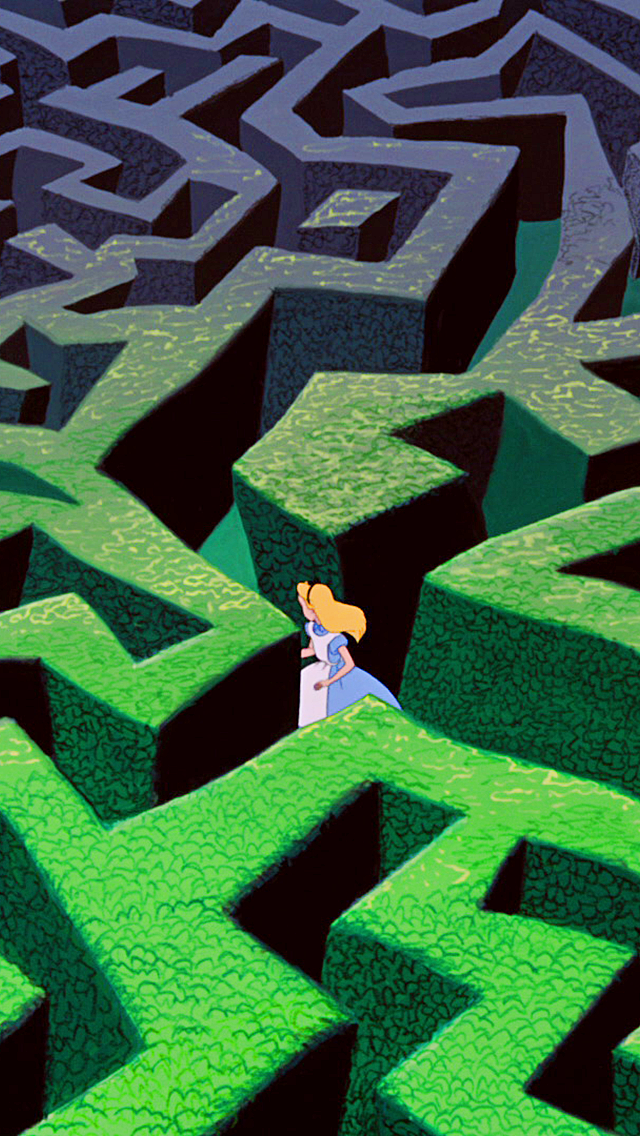
\includegraphics[height=\paperheight]{labyrinth}
      \end{column}
      \begin{column}{0.7\textwidth}
        \Huge\centering Security
      \end{column}
    \end{columns}
  \end{beamercolorbox}
\end{frame}

%%

\begin{frame}{Attacks}
  \begin{block}{Security goal}
    Given the isogeny \emph{$\phi:E\to E$}, the adversary is allowed
    $\poly(T)$ precomputation.

    \bigskip
    Later, it is given a \emph{random $Q\in Y_2$}:\\
    its probability of computing \emph{$\hat\phi(Q)$} in \emph{less
      than ``$T$ steps''} must be negligible.
  \end{block}

  \smallskip
  \emph{Attack avenues:}
  \begin{enumerate}
  \item Speed-up/parallelize isogeny computation;
  \item Solve the pairing equation;
  \item Find isogeny \textit{shortcuts}.
  \end{enumerate}
\end{frame}

%%

\begin{frame}{Attacking the computation?}
  \large
  RSA: \hfill $x \longmapsto x^2\mod N$ \hspace{4em}

  \vfill
  Isogenies: \hfill $\displaystyle x \longmapsto x\frac{x\alpha_i-1}{x-\alpha_i}\mod p$ \hspace{4em}\strut\\
  {\normalsize\color{gray} ($\alpha_1,\dots,\alpha_T$ depend on the chosen isogeny)}

  \vfill
  e.g., \emph{$\quad\log_2 N \approx 2048,\quad \log_2 p \approx 1500$}.
  
  \vfill
  \centering
  No speedup? Even with unlimited parallelism? Really?
  
  \medskip
  See Bernstein, Sorenson. \emph{Modular exponentiation via the
    explicit Chinese remainder theorem}.
\end{frame}

%%

\begin{frame}{Attacking the pairing}
  \large

  A pairing inversion problem:
  \[e(P, \alert{???}) = e(\phi(P), Q)\]

  \bigskip
  \begin{description}
  \item[Quantum:] Broken by Shor's algorithm;
  \item[Classical:] Subexponential \emph{$L_p(1/3)$} attack.\\[1em]
  \item[Note:] Solving the equation gives the \emph{true value of
      $\hat\phi(Q)$} (perfect soundness)
  \end{description}
\end{frame}

%%

\begin{frame}{Computing \textit{shortcuts}}
  \begin{columns}
    \begin{column}{0.5\textwidth}
      \begin{itemize}
      \item Isogeny degree $= \ell^T \leftrightarrow$ \emph{walk length $= T$};
        \begin{itemize}
        \item e.g., for delay $\approx$ 1 hour, \emph{$T\approx 2^{20}$};
        \item<2-> Typically much larger than graph diameter (\emph{$= O(\log p) \approx 2^{10}$}).
        \item<2-> \textcolor{gray}{(which isogeny graph is meant depends on the variant)}
        \end{itemize}
      \item<3-> \emph{Goal:} find a \emph{\textit{shortcut}}, i.e., a
        shorter walk.
      \end{itemize}
    \end{column}
    \begin{column}{0.5\textwidth}
      \centering
      \begin{tikzpicture}[scale=0.3]
        \pgfmathsetseed{2};
        \coordinate (P) at (0,0);
        \draw[red,fill] (P) circle (10pt) +(1,-1) node[auto] {$E$};
        \uncover<2->{
          \foreach \i in {1,...,500} {
            \coordinate (Q) at ($(P) + (380*rand:1)$);
            \draw (P) -- (Q);
            \coordinate (P) at (Q);
          }
          \draw[red,fill] (Q) circle (10pt) +(1.2,0) node[auto] {$E'$};
        }
        \uncover<3->{
          \draw[red] (0,0) edge[->,dashed,bend left,thick] node[auto] {$\psi$} ($(Q)-(10pt,-10pt)$);
        }
      \end{tikzpicture}
    \end{column}
  \end{columns}
\end{frame}

%%

\begin{frame}{$\End(E)$ gives shortcuts}
  \begin{columns}
    \begin{column}{0.48\textwidth}
      \begin{block}{$\F_p$ case}
        \begin{itemize}
        \item \emph{$\End_{\F_p}(E) \subset \Q(\sqrt{-p})$}:\\
          the class group $\Cl(-4p)$ acts on the set of supersingular
          curves $/\F_p$;
        \item \emph{Structure of $\Cl(-4p)$}\\
          $\qquad\Updownarrow$\\
          relations between ideal classes\\
          $\qquad\Updownarrow$\\
          \emph{shortcuts} in the graph.
          \begin{itemize}
          \item see CSI-FiSh signatures (Beullens--Kleinjung--Vercauteren);
          \item akin to attack on \emph{class group VDF}.
          \end{itemize}
        \item Some additional work to find \emph{endomorphism $\omega$}
          such that \emph{$\omega\circ\hat\psi(Q) = \hat\phi(Q)$}.
        \end{itemize}
      \end{block}
    \end{column}
    \pause
    \begin{column}{0.48\textwidth}
      \begin{block}{General case (both $\F_p$ and $\F_{p^2}$)}
        \begin{itemize}
        \item \emph{$\End(E)$} isomorphic to an\\
          \emph{order in a quaternion algebra};
        \item \emph{Structure of $\End(E)$} (or $\End(E')$)\\
          $\qquad\Updownarrow$\\
          \emph{shortcuts} (through $\F_{p^2}$).
          \begin{itemize}
          \item Related to attacks on the Charles--Goren--Lauter hash
            function.
          \end{itemize}
        \item Additional work to find \emph{$\omega\in\End(E)$}.
        \end{itemize}

        \begin{uncoverenv}<3->
          \begin{center}
            \alert{\bf WE HAVE A PROBLEM!}
          \end{center}
          
          No known way to construct supersingular curves
          without knowledge of $\End(E)$.

          \medskip
          Only known fix: \emph{\bf Trusted setup}.

        \end{uncoverenv}
      \end{block}
    \end{column}
  \end{columns}
\end{frame}

%%

\begin{frame}{Trusted setup}
  \begin{columns}
    \begin{column}{0.5\textwidth}
      \centering
      \begin{tikzpicture}[scale=0.2]
        \pgfmathsetseed{2};
        \coordinate (P) at (0,0);
        \draw[red,fill] (P) circle (5pt) +(0,2) node[auto] {$y^2=x^3+x$};
        \uncover<2>{
          \foreach \i in {1,...,100} {
            \coordinate (Q) at ($(P) + (150*rand:1)$);
            \draw (P) -- (Q);
            \coordinate (P) at (Q);
          }
        }
        \uncover<2->{
          \draw[red,fill] (Q) circle (5pt) +(1.2,0) node[auto] {$E$};}
      \end{tikzpicture}
    \end{column}
    \begin{column}{0.5\textwidth}
      \begin{itemize}
      \item<1-> Start from a well known supersingular curve,
      \item<2-> Do a random walk,
      \item<3-> Forget it.
      \end{itemize}
    \end{column}
  \end{columns}

  \begin{uncoverenv}<4->
    \begin{center}
      \begin{tabular}{p{10em} | c c | c c}
        & \multicolumn{2}{c|}{Classical} & \multicolumn{2}{c}{Quantum} \\
        & $\F_p$ graph & $\F_{p^2}$ graph & $\F_p$ graph & $\F_{p^2}$ graph \\
        \hline
        Computing shortcuts & $L_p(1/2)$ & $O(\sqrt{p})$ & $\polylog(p)$ & $O(\sqrt[4]{p})$\\
        Pairing inversion & $L_p(1/3)$ & $L_p(1/3)$ & $\polylog(p)$ & $\polylog(p)$\\
      \end{tabular}
    \end{center}
  
    \emph{\it Quantum annoyance:}
    \begin{itemize}
    \item Computing \emph{shortcuts} in $\F_{p^2}$ is \emph{quantumly
        hard};
    \item Pairing inversion attacks must be run \emph{online}, useless
      if Shor's algorithm takes \emph{much longer than target delay}.
    \end{itemize}
  \end{uncoverenv}
\end{frame}

%%

\begin{frame}{Distributed trusted setups}
  \begin{columns}
    \begin{column}{0.4\textwidth}
      \begin{tikzpicture}[scale=0.2]
        \pgfmathsetseed{2};
        \coordinate (P) at (0,0);
        \draw[red,fill] (P) circle (5pt) +(1,-1) node[auto] {$y^2=x^3+x$};
        \foreach \r in {1,...,3} {
          \coordinate (R) at (P);
          \uncover<+>{
            \foreach \i in {1,...,100} {
              \coordinate (Q) at ($(P) + (360*rand:1)$);
              \draw (P) -- (Q);
              \coordinate (P) at (Q);
            }
          }
          \uncover<.->{
            \draw[red,fill] (Q) circle (5pt) +(1.2,0) node[auto] {$E_\r$};}
          \uncover<+->{
            \draw[dotted] (R) edge[bend right] node[auto,swap] {$\pi_\r$} (Q);}
        }
      \end{tikzpicture}
    \end{column}
    \begin{column}{0.55\textwidth}
      Mitigate trusted setup woes by \emph{distributing trust}:
      \begin{itemize}
      \item<1-> Participant $i$ performs a random walk (in $\F_p$),
      \item<2-> Publishes a \emph{proof} of isogeny knowledge,
      \item<3-> Repeat.
      \end{itemize}

      \smallskip
      \begin{uncoverenv}<7->
        Proof options:
        \begin{itemize}
        \item Generic ZK proofs,
        \item Isogeny ZK proofs (SeaSign),
        \item Pairing proofs (not ZK!):
          \begin{gather*}
            P, Q = \mathcal{H}(E_i,E_{i+1}),\\
            e_i(P,\hat\phi_i(Q)) = e_{i+1}(\phi_i(P),Q).
          \end{gather*}
        \end{itemize}
      
        \smallskip \emph{Properties:} asynchronous, robust against
        $n-1$ coalition, verification scales linearly, updatable,
        \dots
      \end{uncoverenv}
    \end{column}
  \end{columns}
\end{frame}

%%

\begin{frame}[plain]
  \begin{beamercolorbox}[sep=0.1px,center,wd=\paperwidth,ht=\paperheight]{palette tertiary}
    \begin{columns}
      \begin{column}{0.55\textwidth}
        \Huge\centering Beyond VDFs
      \end{column}
      \begin{column}{0.45\textwidth}
        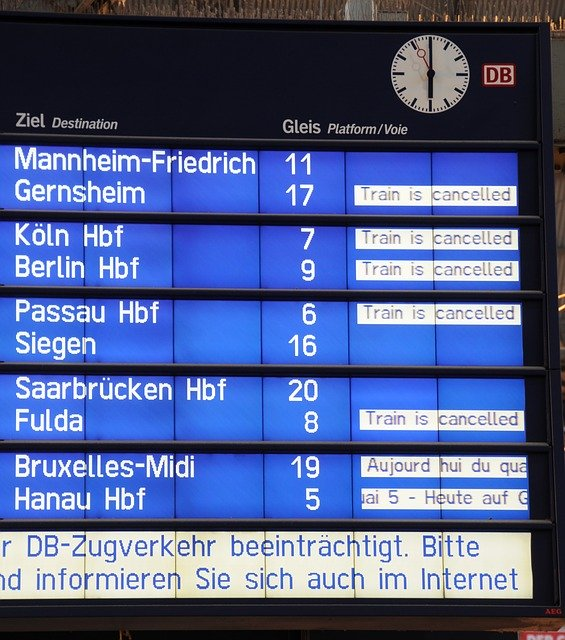
\includegraphics[height=\paperheight]{db.jpg}
      \end{column}
    \end{columns}
  \end{beamercolorbox}
\end{frame}

%%

\begin{frame}{Watermarking}
  \def\Emid{E_{\mathrm{mid}}}
  \def\emid{e_{\mathrm{mid}}}
  \begin{description}
  \item[Goal:] reward evaluator for its effort.
  \item[Watermarking:] issue proof of evaluation \emph{tied to
      evaluator identity}
  \end{description}

  \centering
  \begin{tikzpicture}[x=5cm]
    \node (E) at (0,0) {$E$};
    \node (Em) at (1,0) {$\Emid$};
    \node (E1) at (2,0) {$E'$};
    
    \draw[auto,->] (E1) edge[bend right] node {$\hat\phi_1$} (Em)
    (Em) edge[bend right] node {$\hat\phi_2$} (E)
    (E1) edge[bend left] node[swap] {$\hat\phi = \hat\phi_2\circ\hat\phi_1$} (E);
  \end{tikzpicture}

  \begin{description}
  \item[Secret key:] scalar $s\in\Z/N\Z$,
  \item[Public key:] $s\phi(P) \in E'$ \textcolor{gray}{(+ proof of exponent knowledge)},
  \item[Proof of work:] $s\hat\phi_1(Q) \in \Emid$,
  \item[Verification:] $\emid(\phi_2(P),s\hat\phi_1(Q)) = e'(s\phi(P),Q)$.
  \item[Properties:] blind (can be checked before the computation is
    complete).
  \end{description}
\end{frame}

%%

\begin{frame}{Encryption to the future (time-locks)}
  \begin{description}
  \item[Goal:] encrypt now, decryption only possible after delay.
  \item[Applications:] auctions, voting, \dots
  \item[Idea:] start from Boneh--Franklin IBE, just add
    isogenies\texttrademark.
  \end{description}

  \bigskip
  \centering
  \begin{tabular}{c c c}
    \textbf{Bidder} && \textbf{Auctioneer}\\
                    && Publishes auction key \emph{$Q = \mathcal{H}(\mathsf{sid})$}\\
                    && starts evaluating \emph{$\hat\phi(Q)$}\\
    samples random \emph{$s\in\Z/N\Z$}\\
    computes \emph{$k = e(\phi(P), Q)^s$}\\
    encrypts offer \emph{$o_k = \mathrm{Enc}_{k}(o)$}\\
    \hfill sends \emph{$(o_k,sP)$} & $\longrightarrow$\\
                    && $\vdots$\\
                    && computes \emph{$k = e(sP, \hat\phi(Q))$}\\
                    && decrypts \emph{$o_k$}
  \end{tabular}
\end{frame}

%%

\begin{frame}{Open questions}
  \begin{itemize}
  \item<+-> Understand the impact of large memory requirements in
    evaluation; is a time/memory trade-off reasonable?
  \item<+-> Remove trusted setup:
    \begin{itemize}
    \item Hash into the supersingular set, or
    \item Construct ordinary pairing friendly curves with large
      discriminant.
    \end{itemize}
  \item<+-> Explore more advanced pairing+delay constructions.
  \item<+-> Spend millions on dedicated hardware for $2$-isogenies.
  \end{itemize}

  \bigskip
  \begin{uncoverenv}<+->
    \begin{center}
      \Large Just Add Isogenies\texttrademark!
    \end{center}
  \end{uncoverenv}
\end{frame}

%%

\begin{frame}[plain]
  \centering
  \begin{tikzpicture}[remember picture,overlay]
    \begin{scope}[xscale=1.7,yshift=-15,opacity=0.8]
      \def\crater{12}
      \def\jumpa{-8}
      \def\jumpb{9}
      \def\diam{5cm}

      \foreach \i in {1,...,\crater} {
        \draw[blue] (360/\crater*\i : \diam) to[bend right] (360/\crater*\i+360/\crater : \diam);
        \draw[red] (360/\crater*\i : \diam) to[bend right] (360/\crater*\i+\jumpa*360/\crater : \diam);
        \draw[green] (360/\crater*\i : \diam) to[bend right=50] (360/\crater*\i+\jumpb*360/\crater : \diam);
      }
    \end{scope}
    
    \draw (0,0.5) node{\Huge\bf Thank you};
    \draw (0,-1.1) node{\large\url{https://defeo.lu/}};
    \draw (0,-1.8) node{\large
\includegraphics[height=0.9em]{twitter.png}~\href{https://twitter.com/luca_defeo}{@luca\_defeo}};
  \end{tikzpicture}
\end{frame}

\end{document}


% LocalWords:  Isogeny abelian isogenies hyperelliptic supersingular Frobenius
% LocalWords:  isogenous
